% system_design.tex
%
% Subsections:
%   3.1  Core Abstraction
%   3.2  Execution Environment
%   3.3  Evaluation Pipeline
%   3.4  Search Strategies
%   3.5  Architecture Overview (diagram)

\section{System Design}
\label{sec:system-design}

\textsc{anneal} is a framework for LLM-guided artifact optimization.
An \emph{artifact} is any text-based software object that can be evaluated
for quality: a system prompt, a Python function, a configuration file,
or a technical document.
\textsc{anneal} treats the artifact as the subject of optimization, an
\emph{evaluation function} as the objective, and an \emph{LLM agent} as the
mutation operator.

% --- 3.1 Core Abstraction ---
\subsection{Core Abstraction: Artifact--Eval--Agent Triplet}
\label{sec:design-abstraction}

% Describe the three-component model:
%   - Artifact: versioned text object stored in a git-tracked workspace
%   - Eval: deterministic function or stochastic LLM judge
%   - Agent: LLM mutation operator (dual-agent: critic + writer)
\TODO{Write this subsection. Include:
  (1) Formal definition of artifact, eval function, mutation operator.
  (2) How the triplet composes into an optimization loop.
  (3) What ``artifact-agnostic'' means in practice.}

The core optimization loop is:
\begin{equation}
  a_{t+1} = \mathrm{Mutate}(a_t,\, \mathcal{H}_t,\, \mathcal{K}_t)
  \label{eq:mutation}
\end{equation}
where $a_t$ is the current artifact at step $t$,
$\mathcal{H}_t$ is the lineage history (previous artifacts and their scores),
and $\mathcal{K}_t$ is the accumulated knowledge pool.
A candidate $a_{t+1}$ is accepted if it scores significantly higher than $a_t$
under a Wilcoxon signed-rank test (\cref{sec:enhancements-eval}).

% --- 3.2 Execution Environment ---
\subsection{Execution Environment: Git Worktree Isolation}
\label{sec:design-worktree}

% Describe git worktree isolation:
%   - Each optimization run gets its own worktree
%   - No shared mutable state between parallel runs
%   - Enables reproducibility: every artifact version is addressable by commit hash
\TODO{Write this subsection. Explain why worktree isolation matters for:
  (1) reproducibility,
  (2) parallel execution of multiple runs,
  (3) audit trail (git history = optimization history).}

% --- 3.3 Evaluation Pipeline ---
\subsection{Evaluation Pipeline}
\label{sec:design-eval}

\TODO{Write this subsection covering:
  (1) Deterministic eval: pure functions returning scalar scores.
  (2) Stochastic eval: LLM judge with multiple samples.
  (3) Evaluation caching: SHA256 content hash over artifact + eval config.
  (4) Bradley-Terry scoring for multi-criteria aggregation.
  (5) Adaptive sampling: stop early when confidence interval is tight enough.}

% Figure: evaluation pipeline schematic
\begin{figure}[h]
  \centering
  % \includegraphics[width=\linewidth]{figures/eval_pipeline.pdf}
  \TODO{Insert evaluation pipeline figure. Show: artifact -> eval function
    -> score samples -> Bradley-Terry aggregation -> acceptance test.}
  \caption{The \textsc{anneal} evaluation pipeline. Stochastic evaluators
    sample the LLM judge multiple times; adaptive sampling halts when the
    Bradley-Terry score estimate reaches a target confidence interval.
    Results are cached by content hash to avoid redundant evaluation.}
  \label{fig:eval-pipeline}
\end{figure}

% --- 3.4 Search Strategies ---
\subsection{Search Strategies}
\label{sec:design-search}

% Describe the strategy abstraction and the strategies implemented:
%   - Greedy: always mutate the current best
%   - Pareto: maintain non-dominated front for multi-objective
%   - Island: maintain diverse population, periodic migration
%   - Thompson Sampling: select strategy via beta-binomial bandit
\TODO{Write this subsection. Enumerate strategies and their selection policy.
Reference the StrategyManifest introduced in the enhancements section.}

% --- 3.5 Architecture Overview ---
\subsection{Architecture Overview}
\label{sec:design-architecture}

\TODO{Write this subsection as a high-level narrative accompanying the
architecture diagram.}

% Figure: full architecture diagram
\begin{figure}[h]
  \centering
  % 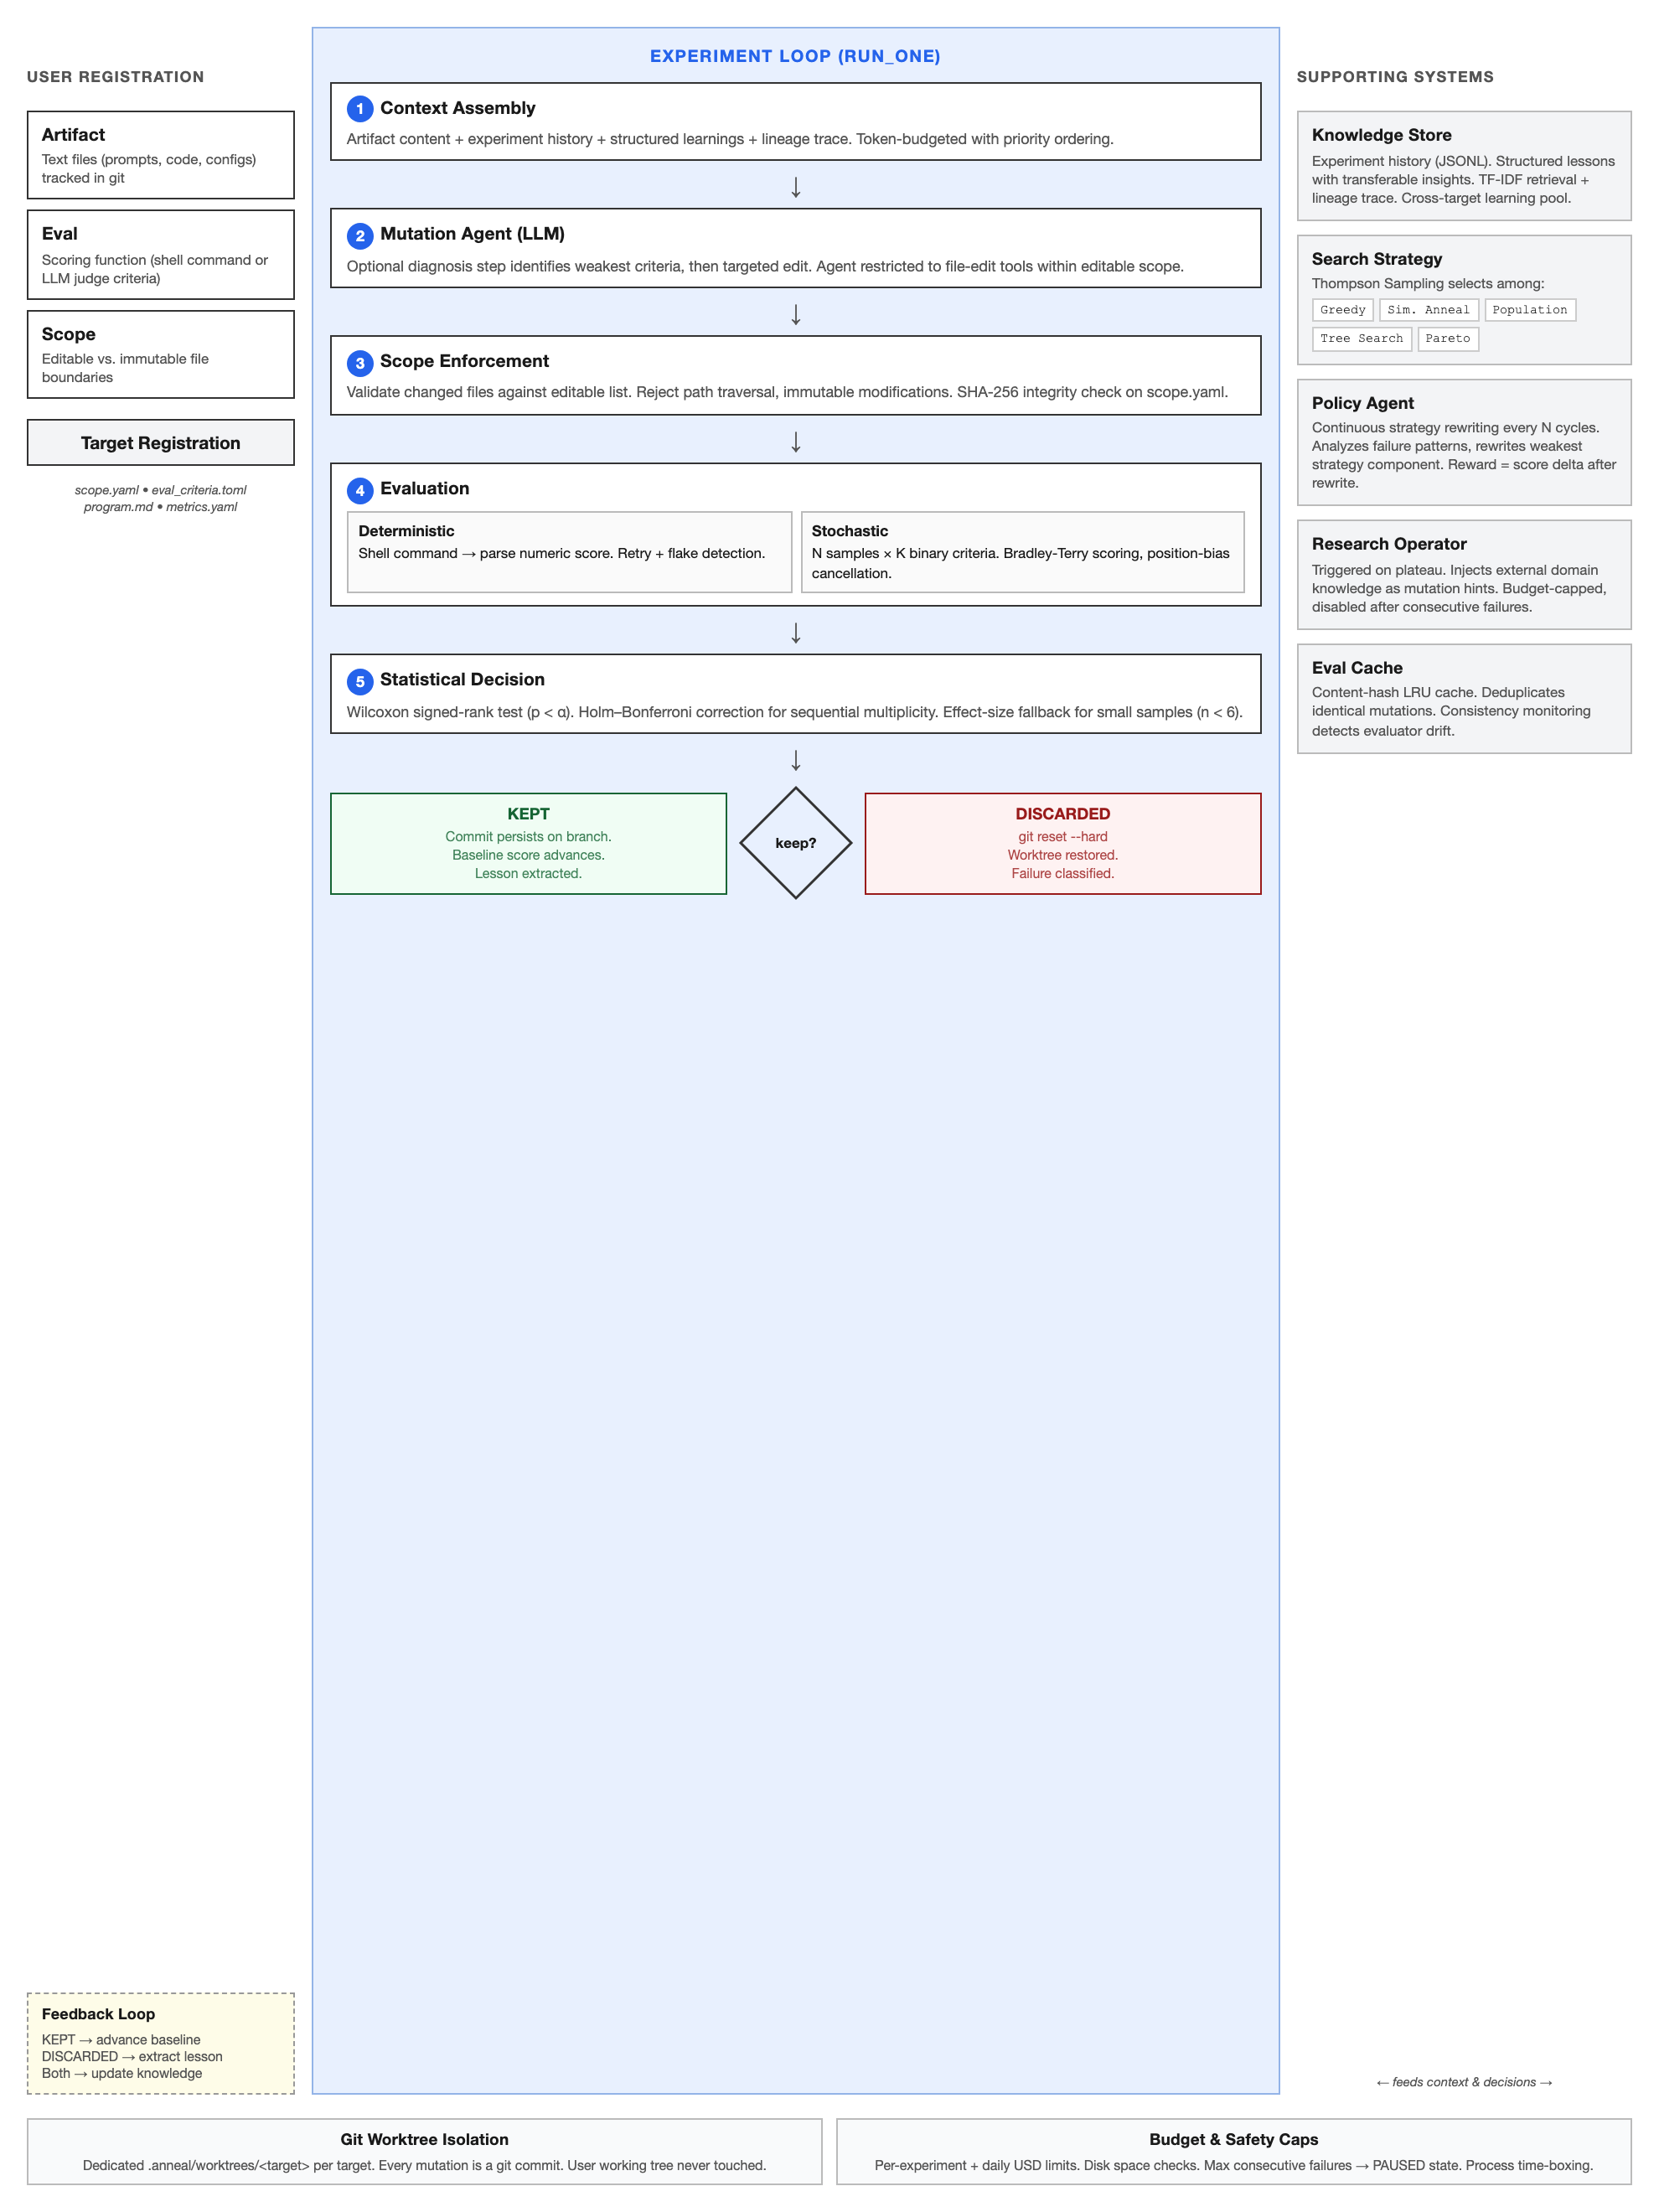
\includegraphics[width=\linewidth]{figures/architecture.pdf}
  \TODO{Insert architecture diagram. Components: CLI, Runner, Search Engine,
    Eval Engine, Knowledge Pool, Strategy Selector, Git Worktree Manager.
    Show data flow and control flow as separate arrow styles.}
  \caption{Architecture of \textsc{anneal}. The runner orchestrates the
    optimization loop, delegating mutation to the dual-agent pair,
    evaluation to the eval engine (with caching), and strategy selection
    to the Thompson Sampling bandit. The knowledge pool persists across
    optimization runs and is queried during context construction.}
  \label{fig:architecture}
\end{figure}
